\section{Вычисление опорных функций}

В наших рассуждениях важную роль играет выпуклая функция, которая называется опорной функцией множества.
Рассмотрим $\R^n$~--- евклидово пространство и $X$~--- его непустое подмножество.

\begin{definition}
        \textit{Опорная функция} множества $X \subset \R^n$ определена на $\R^n$ соотношением
        $$
                \rho(l\,|\,X) = \sup\limits_{x \in X} \langle l,\,x\rangle,\quad l \in \R^n.
        $$
\end{definition}

\subsection{Вычисление опорной функции множества $\X_0$}

Напомним, что множество $\X_0 = B_r(x_0)$, то есть шар радиуса $r > 0$ с центром в точке $x_0$.
Видно, что данное множество можно разложить в сумму двух множеств по Минковскому:
$$
        \X_0 = B_r(x_0) = B_r(0) + \{\,x_0\,\}.
$$

\begin{assertion}
        Опорная функция аддитивна по второму аргументу:
        $$
                \rho(l\,|\,A + B) = \rho(l\,|\,A) + \rho(l\,|\, B), 
        $$
        где под $A + B$ понимается сумма Минковского
        $
                A + B :=\{\,a+b \in \R^n \;:\; a \in A,\,b \in B\,\}.
        $
\end{assertion}
\begin{proof}
        Приведём простейшую цепочку преобразований:
        \begin{multline*}
                \rho(l\,|\,A + B) = \sup\limits_{x \in A + B}\langle l,\,x\rangle = \sup\limits_{a \in A,\,b \in B}\langle l,\,a + b\rangle =\\= \sup\limits_{a \in A}\langle l,\,a \rangle + \sup\limits_{b \in B}\langle l,\,b\rangle = \rho(l\,|\,A) + \rho(l\,|\,B).
        \end{multline*}
\end{proof}

Тогда, очевидно, опорная функция множества $\X_0$ имеет вид:
\begin{equation}\label{eq:support_x0}
        \boxed{
                \rho(l\,|\,\X_0) = \langle l,\,x_0\rangle + r|\,l\,|
        }.
\end{equation}


\subsection{Вычисление опорной функции множества $\X_1$}

Напомним, что множество $\X_1$ имеет вид
$$
        \X_1 = \{\, x \in \R^2\;:\; Gx + g \leqslant 0\,\},\quad G \in \R^{m\times 2},\,g\in \R^{m},\,m\in\N,
$$
то есть задаётся пересечением множеств, задаваемых неравенствами:
$$
        G_{i1}x_1 + G_{i2}x_2 \leqslant -g_i,\quad i = \overline{1,\,m}.
$$

Каждое из неравенств представляет собой полуплоскоть, ограниченную линейной функцией $x_2 = -\frac{G_{i1}}{G_{i2}} - \frac{g_i}{G_{i2}}$.
Рассмотрим возможные пересечения таких множеств:
\begin{description}
        \item[Пустое множество.] Действительно, можно подобрать параметры, при которых множество $\X_1$ будет пустым. Например, при
        $$
                G =
                \begin{pmatrix}
                         1 &  1 \\
                        -1 & -1 
                \end{pmatrix}
                ,\quad
                g =
                \begin{pmatrix}
                        0 \\
                        1
                \end{pmatrix}
                .
        $$
        Этот случай нас не интересует, так как при таких условиях поставленная задача не имеет смысла.
        \item[Полуплоскость.] Приведём пример полуплоскости:
        $$
                G =
                \begin{pmatrix}
                        1 & 1
                \end{pmatrix}
                ,\quad
                g =
                \begin{pmatrix}
                        1
                \end{pmatrix}.
        $$
        Пусть полуплоскость задана неравенством $\alpha x_1 + \beta x_2 \leqslant \gamma$, тогда
        $$
                \rho(l\,|\,\X_1) =
                \begin{cases}
                        \frac\gamma\beta l_2, & l = (\alpha,\,\beta)^\T \\
                        +\infty, & \mbox{иначе.}
                \end{cases}
        $$
        \item[Полоса.] Назовём полосой множество, лежащее между двумя параллельными прямыми на плоскости. Такая ситуация возможна, например, при
        $$
                G =
                \begin{pmatrix}
                         1 &  1 \\
                        -1 & -1 
                \end{pmatrix}
                ,\quad
                g =
                \begin{pmatrix}
                        1 \\
                        0
                \end{pmatrix}
                .
        $$
        Пусть множество задано прямыми $\alpha x_1 + \beta x_2 = \gamma_1$ и $-\alpha x_1 - \beta x_2 =\gamma_2$. Тогда
        $$
                \rho(l\,|\,\X_1) =
                \begin{cases}
                        \frac{\gamma_1}\beta l_2, & l = (\alpha,\,\beta)^\T \\
                        \frac{\gamma_2}\beta l_2, & l = (-\alpha,\,-\beta)^\T \\
                        +\infty, & \mbox{иначе.}
                \end{cases}
        $$
        \item[Прямая.] Действительно, можно подобрать параметры так, чтобы множество $\X_1$ вырождалось в прямую. Например, при
        $$
                G =
                \begin{pmatrix}
                         1 &  1 \\
                        -1 & -1 
                \end{pmatrix}
                ,\quad
                g =
                \begin{pmatrix}
                        0 \\
                        0
                \end{pmatrix}
                .    
        $$
        Пусть прямая задана уравнением $\alpha x_1 + \beta x_2 = \gamma$, тогда
        $$
                \rho(l\,|\,\X_1) =
                \begin{cases}
                        \frac\gamma\beta l_2, & l = \pm(\alpha,\,\beta)^\T \\
                        +\infty, & \mbox{иначе.}
                \end{cases}
        $$
        \item[Множество с кусочно-линейной границей.] Действительно, при последовательном отсечении от множества конечного числа полуплоскостей, очевидно, получается множество, граница которого представляет собой объединение конечного отрезков или прямых. Рассмотрим этот случай более подробно.
\end{description}

Докажем, что множество $\X_1$ является выпуклым. В этом нам поможет следующее утверждение.
\begin{assertion}
        Пересечение любого числа выпуклых множеств $X_\sigma \subset \R^n$, $\sigma \in \Sigma$ является выпуклым множеством.
\end{assertion}
\begin{proof}
        Возьмём произвольные точки $x,\,y \in \bigcap\limits_{\sigma \in \Sigma} X_\sigma$. Каждое из множеств $X_\sigma$ является выпуклым. Поэтому $[x,\,y] \subset X_\sigma$ для любого $\sigma \in \Sigma$. Отсюда $[x,\,y] \in \bigcap\limits_{\sigma \in \Sigma} X_\sigma$. Что по определению означает выпуклость пересечения множеств $\bigcap\limits_{\sigma \in \Sigma} X_\sigma$.
\end{proof} 

Введём важное для нашей работы понятие крайней точки выпуклого множества. Пусть $X \subset \R^n$~--- выпуклое замкнутое множество.
\begin{definition}
        Точка $x_0 \in X$ называется \textit{крайней точкой множества $X$} , если не существует таких точек $x_1,\,x_2 \in A$, $x_1 \neq x_2$ , что $x_0 \in (x_1,\,x_2)$ (то есть $x_0 = \alpha x_1 + (1-\alpha)x_2$ для некоторого $\alpha\;:\; 0 < \alpha < 1$). Множество крайних точек множества $X$ обозначается через ext($X$).
\end{definition}

\begin{assertion}
        Множество $\X_1$~--- выпуклое и замкнутое.
\end{assertion}
Доказательство этого факта опирается на то, что множество $\X_1$ является пересечением полуплоскостей, каждая из которых, очевидно, выпуклое и замкнутое множество. Пересечение же замкнутых и выпуклых множеств, как известно, также замкнутое и выпуклое множество соответственно.

\begin{equation} \label{eq:support_x1}
\boxed {
        \rho(l\,|\,\X_1) =
        \begin{cases}
                \max\limits_{x \in \mathrm{ext}\X_1} \langle l,\, x \rangle,
                & \mbox{если $\nexists \,\varepsilon > 0 \,:\, \mathrm{argmax}_{x \in \mathrm{ext}\X_1}\langle l,\, x \rangle + \varepsilon l \in \X_1$}
                \\
                +\infty, &\mbox{иначе.}
        \end{cases}        
}
\end{equation}

\subsection{Вычисление опорной функции множества $\Omega$}

Заметим, что множество
$$
        \Omega = \{\,x = (x_1,\,x_2)^\T \in \R^2 \;:\; ax_1^2 \leqslant x_2 \leqslant b - cx_1^2\,\},\quad a,\,b,\,c > 0
$$
является пересечением двух множеств:
$$
\begin{aligned}
        &\Omega_1 = \{\,x = (x_1,\,x_2)^\T \in \R^2 \;:\; ax_1^2 \leqslant x_2\,\},\quad &a > 0,\\
        &\Omega_2 = \{\,x = (x_1,\,x_2)^\T \in \R^2 \;:\;  x_2 \leqslant b - cx_1^2\,\},\quad &b,\,c > 0.
\end{aligned}
$$
Введём следующие обозначения:
$$
\begin{aligned}
        x_{11} &= \sqrt{\frac{b}{a+c}},\\
        x_{12} &= -x_{11},\\
        x_{20} &= \frac{ab}{a+c}.
\end{aligned}
$$
Также отметим, что $(x_{11},\,x_{20})$ и $(x_{12},\,x_{20})$ являются точками пересечения парабол $ax_1^2 = x_2$ и $b - cx_1^2 = x_2$.
При $l_2 \leqslant 0$ имеет смысл рассматривать множество $\Omega_1$ с ограничением $x_2 \leqslant x_{20}$, а при $l_2 \geqslant 0$~--- $\Omega_2$ с ограничением $x_2 \geqslant x_{20}$.

\begin{figure}[h]
\center{
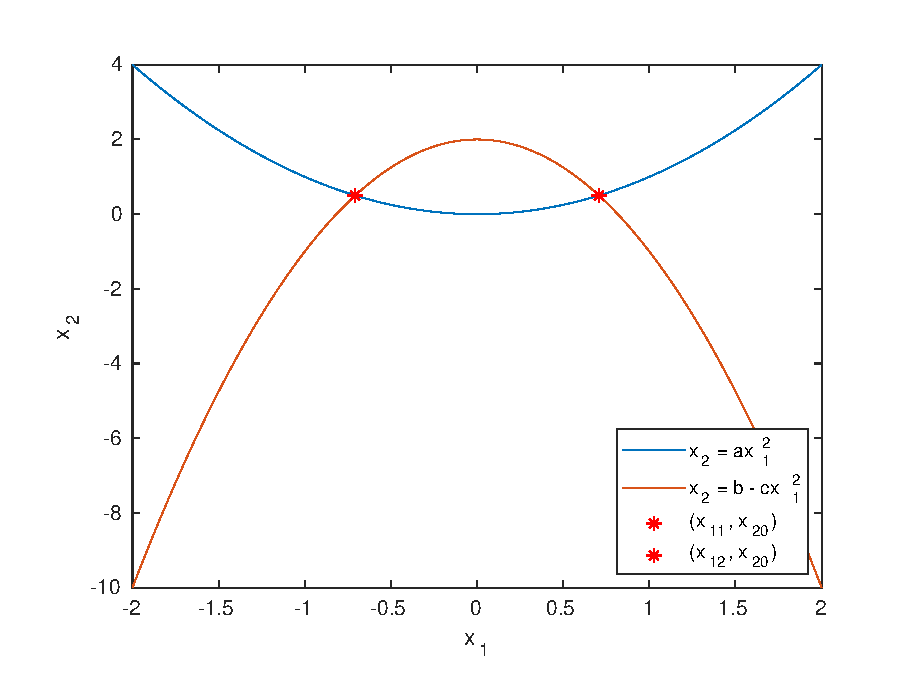
\includegraphics[width=0.5\textwidth]{support_functions/omega.eps}}
\caption{Уравнения, ограничивающие множество $\Omega$.}
\end{figure}

Посчитаем опорную функцию множества $\Omega_1$ при $l_2 \leqslant 0$:
$$
        \rho(l\,|\,\Omega_1) = 
        \sup\limits_{x \in \Omega_1}\langle x,\,l\rangle =
        \sup\limits_{x \in \Omega_1} (x_1l_1 + x_2l_2) =
        \sup\limits_{x \in \Omega_1}(x_1l_1 + ax_1^2l_2).
$$
Найдём экстремум по $x_1$:
$$
        (x_1l_1 + ax_1^2l_2)' = 0
$$
$$
        l_1 - 2ax_1l_2 = 0
$$
$$
        x_1 = \frac{l_1}{2al_2},
$$
откуда $x_2 = ax_1^2 = \frac{l_1^2}{4al_2^2}$.

Посчитаем опорную функцию множества $\Omega_2$ при $l_2 \geqslant 0$:
$$
\rho(l\,|\,\Omega_2) = 
        \sup\limits_{x \in \Omega_2}\langle x,\,l\rangle =
        \sup\limits_{x \in \Omega_2} (x_1l_1 + x_2l_2) =
        \sup\limits_{x \in \Omega_2}(x_1l_1 + b - cx_1^2l_2).
$$
Найдем экстремум по $x_1$:
$$
        (x_1l_1 + b - cx_1^2l_2)' = 0
$$
$$
        l_1 - 2cx_1l_2 = 0
$$
$$
        x_1 = \frac{l_1}{2cl_2},
$$
откуда $x_2 = b - cx_1^2 = b - \frac{l_1^2}{4cl_2^2}$.

Подведём итог:
\begin{equation}\label{eq:support_omega}
\boxed{
\begin{aligned}
        \rho(l\,|\,\Omega) =
        \left\{
        \begin{aligned}
        &\frac{l_1^2}{2al_2} + \frac{l_1^2}{4al_2}, && \mbox{при $l_2 \leqslant 0$, $\frac{l_1^2}{4al_2^2} \leqslant x_{20}$} \\
        &x_{12}l_1 + x_{20}l_2, && \mbox{при $l_2 \leqslant 0$, $\frac{l_1^2}{4al_2^2} > x_{20}$, $l_1 < 0$} \\
        &x_{11}l_1 + x_{20}l_2, && \mbox{при $l_2 \leqslant 0$, $\frac{l_1^2}{4al_2^2} > x_{20}$, $l_1 > 0$} \\
        &\frac{l_1^2}{2cl_2} + \left(b - \frac{l_1^2}{4cl_2^2}\right)l_2, && \mbox{при $l_2 \geqslant 0$, $b - \frac{l_1^2}{4cl_2^2} \geqslant x_{20}$} \\
        &x_{12}l_1 + x_{20}l_2, && \mbox{при $l_2 \geqslant 0$, $b - \frac{l_1^2}{4cl_2^2} < x_{20}$, $l_1 < 0$} \\
        &x_{11}l_1 + x_{20}l_2, && \mbox{при $l_2 \geqslant 0$, $b - \frac{l_1^2}{4cl_2^2} < x_{20}$, $l_1 > 0$}.
        \end{aligned}
        \right.
\end{aligned}
}
\end{equation}
Максимизатором является элемент
$$
        x =
        \left\{
        \begin{aligned}
        &\left[\frac{l_1^2}{2al_2},\,\frac{l_1^2}{4al_2^2}\right]^\T, && \mbox{при $l_2 \leqslant 0$, $\frac{l_1^2}{4al_2^2} \leqslant x_{20}$} \\
        &\;[x_{12},\,x_{20}]^\T, && \mbox{при $l_2 \leqslant 0$, $\frac{l_1^2}{4al_2^2} > x_{20}$, $l_1 < 0$} \\
        &\;[x_{11},\,x_{20}]^\T, && \mbox{при $l_2 \leqslant 0$, $\frac{l_1^2}{4al_2^2} > x_{20}$, $l_1 > 0$} \\
        &\left[\frac{l_1}{2cl_2},\, b - \frac{l_1^2}{4cl_2^2}\right]^\T, && \mbox{при $l_2 \geqslant 0$, $b - \frac{l_1^2}{4cl_2^2} \geqslant x_{20}$} \\
        &\;[x_{12},\,x_{20}]^\T, && \mbox{при $l_2 \geqslant 0$, $b - \frac{l_1^2}{4cl_2^2} < x_{20}$, $l_1 < 0$} \\
        &\;[x_{11},\,x_{20}]^\T, && \mbox{при $l_2 \geqslant 0$, $b - \frac{l_1^2}{4cl_2^2} < x_{20}$, $l_1 > 0$}.
        \end{aligned}
        \right.
$$

